\documentclass[../main.tex]{subfiles}

\begin{document}

\chapter{Основные используемые определения}


В данной главе будут введены основные определения и описана формальная постановка задачи. Под желаемым результатом мы далее будем понимать максимизацию некоторой скалярной величины, называемой \emph{наградой} (reward). Интеллектуальную сущность (систему/робота/алгоритм), принимающую решения, будем называть \emph{агентом} (agent). Агент взаимодействует с  \emph{средой} (environment), которая задаётся зависящим от времени \emph{состоянием} (state). Агенту в каждый момент времени в общем случае доступно только некоторое \emph{наблюдение} (observation) текущего состояния мира. Сам агент задаёт процедуру выбора \emph{действия} (action) по доступным наблюдениям; эту процедуру далее будем называть \emph{стратегией}  (policy). Процесс взаимодействия агента и среды задаётся \emph{динамикой среды} (world dynamics), определяющей правила смены состояний среды во времени и генерации награды.

Буквы $s$, $a$, $r$ зарезервируем для состояний, действий и наград соответственно; буквой $t$ будем обозначать время в процессе взаимодействия. 

%\import{1.Setup/}{1.1.MDP.tex}
\section{Основные определения из RL}



\emph{Средой} (environment) называется тройка $(\St, \A, \Trans)$, где: 
\begin{itemize}
	\item $\St$ --- \emph{пространство состояний} (state space), некоторое множество.
	\item $\A$ --- \emph{пространство действий} (action space), некоторое множество.
	\item $\Trans$ --- \emph{функция переходов} (transition function) или \emph{динамика среды} (world dynamics): вероятности $p(s' \HM\mid s, a)$.
\end{itemize}

Набор $\Traj \coloneqq \left( s_0, a_0, s_1, a_1, s_2, a_2, s_3, a_3 \dots \right) $ называется \emph{траекторией}.


\emph{Стратегия(политика)} - распределение $\pi(a \mid s), a \HM\in \A, s \HM\in \St$.


Для данной среды, политики $\pi$ и начального состояния $s_0 \HM\in \St$ распределение, из которого приходят траектории $\Traj$, называется \emph{trajectory distribution}:
$$p\left(\Traj \right) = p(a_0, s_1, a_1 \dots) = \prod_{t \ge 0} \pi(a_t \mid s_t) p(s_{t+1} \mid s_t, a_t)$$



\begin{equation}\label{traj_expectation}
\E_{\Traj} \left( \cdot \right) \coloneqq \E_{\pi(a_0 \mid s_0)}\E_{p(s_1 \mid s_0, a_0)}\E_{\pi(a_1 \mid s_1)} \dots \left( \cdot \right)
\end{equation}

Поскольку часто придётся раскладывать эту цепочку, договоримся о следующем сокращении:
$$\E_{\Traj} \left( \cdot \right) = \E_{a_0}\E_{s_1}\E_{a_1} \dots \left( \cdot \right)$$

Однако в такой записи стоит помнить, что действия приходят из некоторой зафиксированной политики $\pi$, которая неявно присутствует в выражении. Для напоминания об этом будет, где уместно, использоваться запись $\E_{\Traj \sim \pi}$.



\needspace{7\baselineskip}
\begin{wrapfigure}{r}{0.25\textwidth}
	\vspace{-0.4cm}
	\centering
	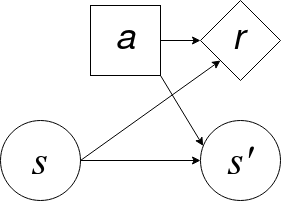
\includegraphics[width=0.15\textwidth]{Images/MDP.drawio.png}
	
	\vspace{-0.8cm}
\end{wrapfigure}


	\emph{Марковский процесс принятия решений} (Markov Decision Process, MDP) --- это четвёрка $(\St, \A, \Trans, r)$, где: 
	
	
	
	\begin{itemize}
		\item $\St, \A, \Trans$ --- среда.
		\item $r: \St \times \A \to \R$ --- \emph{функция награды} (reward function).
	\end{itemize}


%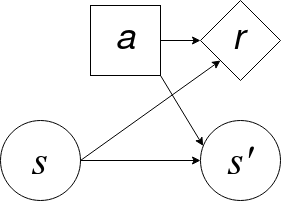
\includegraphics[width=0.15\textwidth]{Images/MDP.drawio.png}



	\emph{Дисконтированной кумулятивной наградой} (discounted cumulative reward) или \emph{total return} для траектории $\Traj$ с коэффициентом $\gamma \HM\in (0, 1]$ называется
	\begin{equation}\label{return}
	R(\Traj) \coloneqq \sum_{t \ge 0} \gamma^t r(s_t, a_t)
	\end{equation}




	Для траектории $\Traj$ величина
	\begin{equation}\label{rewardtogo}
	R_t \coloneqq R \left( \Traj_{t:} \right) = \sum_{\hat{t} \ge t} \gamma^{\hat{t} - t} r_{\hat{t}}
	\end{equation}
	называется \emph{reward-to-go} с момента времени $t$.


\begin{definition}
	\emph{Скором} (score или performance) стратегии $\pi$ в данном MDP называется
	\begin{equation}\label{goal}
	J(\pi) \coloneqq \E_{\Traj \sim \pi} R(\Traj)
	\end{equation}
\end{definition}

Итак, задачей обучения с подкреплением является оптимизация для заданного MDP средней дисконтированной кумулятивной награды:
\begin{equation*}
	J(\pi) \to \max_{\pi}
\end{equation*}

\begin{definition} 
	Для данного MDP \emph{V-функцией} (value function) или оценочной функцией состояний (state value function) для данной стратегии $\pi$ называется величина 
	\begin{equation}\label{Vdefinition}
	V^\pi(s) \coloneqq \E_{\Traj \sim \pi \mid s_0 = s} R \left( \Traj \right)
	\end{equation}
\end{definition}

\begin{definition} 
	Для данного MDP \emph{Q-функцией} (state-action value function, action quality function) для данной стратегии $\pi$ называется
	$$Q^\pi(s, a) \coloneqq \E_{\Traj \sim \pi \mid s_0 = s, a_0 = a} \sum_{t \ge 0} \gamma^t r_t$$
\end{definition}

\begin{definition} 
	Для данного MDP \emph{Advantage-функцией} политики $\pi$ называется
	\begin{equation}\label{advantage}
	A^\pi(s, a) \coloneqq Q^\pi(s, a) - V^\pi(s)
	\end{equation}
\end{definition}


%\import{1.Setup/}{1.2.POMDP.tex}

\section{Частично наблюдаемый MDP}


Частично наблюдаемые MDP являются математическим инструментом для моделирования процесса принятия решения в ситуациях, когда результат зависит как от случайности, заложенной  в самой среде, так и от отсутствия агента полной информации об этой среде.

%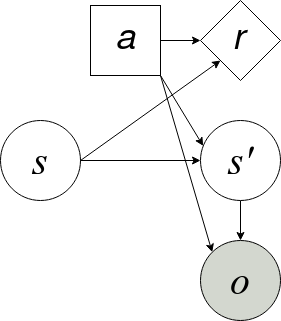
\includegraphics[width=0.15\textwidth]{Images/PoMDP.drawio.png}
\needspace{9\baselineskip}
\begin{wrapfigure}{r}{0.25\textwidth}
	\vspace{-0.4cm}
	\centering
	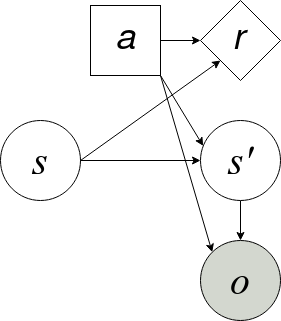
\includegraphics[width=0.15\textwidth]{Images/PoMDP.drawio.png}
	\vspace{-0.4cm}
\end{wrapfigure}
\needspace{7\baselineskip}

%\begin{definition}
	MDP называется \emph{частично наблюдаемым} (partially observable, принятое сокращение --- PoMDP), если дополнительно задано множество $\mathcal{O}$, называемое \emph{пространством наблюдений} (observation space), и распределение $p(o \mid s', a)$, определяющая вероятность получить то или иное наблюдение агента $o \in \mathcal{O}$ в момент времени, когда мир находится в состоянии $s' \in \St$, в которое он попал при выполнении агентом действия $a$.
	\begin{itemize}
		\item $(\St, \A, \Trans, r)$ --- Марковский процесс принятия решений.
		\item $\mathcal{O}$ --- пространство наблюдений.
		\item $p(o \mid s', a)$ --- \emph{распределение наблюдений} (observation function).
	\end{itemize}
%\end{definition}



Также как и для случая наблюдаемого MDP, задачей обучения с подкреплением в PoMDP является
\begin{equation*}
	\E_{\Traj \sim \pi} \sum_{t \ge 0} \gamma^t r(s_t, a_t) \to \max_{\pi}
\end{equation*} 


Препятствием для использования классических методов RL к POMDP является то, что агенту неизвестно состояние среды $s$, на основе которого в  случае наблюдаемого MDP агент получал бы распределение вероятностей по действиям в $\pi(a \mid s)$. Состояние $s$ важно тем, что в оптимизируемом функционале \eqref{goal} функция $r$ для каждого момента времени $t$ помимо действия $_ta$ зависит именно от $s_t$, а сумма функций для всех последующих моментов времени $\hat{t} \ge t$ зависит от соответствующих состояний $s_{\hat{t}}$, вероятность попадания которых также определяется состоянием $s_t$.


Возможным решением здесь тогда будет переход от построения стратегии на основе состояния к стратегии на основе некторой информации, известной нам о состоянии.
Это может быть достигнуто применением Байесовской статистики --- теории в области статистики,основанной на Байесовской интерпретации вероятности, когда вероятность отражает степень доверия событию, которая может измениться, когда будет собрана новая информация. В этом случае PoMDP рассматривается в виде графовой вероятностной  модели --- Байесовской сети (Bayesian Networks), где каждой вершине ориентированного графа соответствует случайная переменная, а дуге --- зависимость между этими переменными. 

  
Тогда состояние  $s$ заменяется распределением вероятностей по $s$, отражающим степень доверия к состоянию --- \emph{belief}. Так в случае конечного пространства состояний $\St$ скалярное значение состояния $s$ заменяется на вектор размерности  $|\St|$. 

Следует отметить, что указанное распределение вероятностей является обусловленным всей уже известной агенту информацией --- последовательностью его наблюдений и действий,  называемой историей агента (action-observation history). 

\begin{definition}
	Последовательность наблюдений и действий агента до момента $t$ называется историей агента
	$h_t = (o_0, a_0, o_1, a_1, \dots ,a_{t-1}, o_t)$
\end{definition}

Фактически история является "обрезанной" до момента $t$ траекторией, но ввиду важности ее использования в стратегиях для PoMDP имеет смысл использовать отдельное определение и обозначение. История может задаваться рекурсивно следующим выражением
\begin{equation}
\label{update_history}
\begin{cases}
h_0 = o_0 \\
h_{t+1} = <h_{t}, a_{t}, o_{t+1}>
\end{cases}
\end{equation}

\begin{definition}
	Вероятность пребывания в том или ином состоянии при условии наблюдаемой истории  называется \emph{belief state} 
	$$b_t = p(s_t \HM\mid h_{t})$$
	\end{definition}

	Рассмотрение процесса в виде Байесовской сети, относящейся без учета функции награды к расширению скрытой марковской цепи  --- input output HMM, и анализа условной независимости, представленной здесь графическим свойством d-разделённости (d-separation), позволяет обосновать недостаточность использования только последнего наблюдения в качестве входного значения стратегии. 

\begin{multicols}{2}[\columnsep2em] 

	
	Для этого необходимо выделить три множества случайных величин и соответствующих им   вершин графа:
	\begin{itemize}
		\item $A=\{ s_t\}$ 
		\item $B=h_{t-1} = \{a_0, o_1,... , a_{t-2}, o_{t-1}\}$ 
		\item $C=\{ a_{t-1}, o_t \}$ 
	\end{itemize}
	\columnbreak
	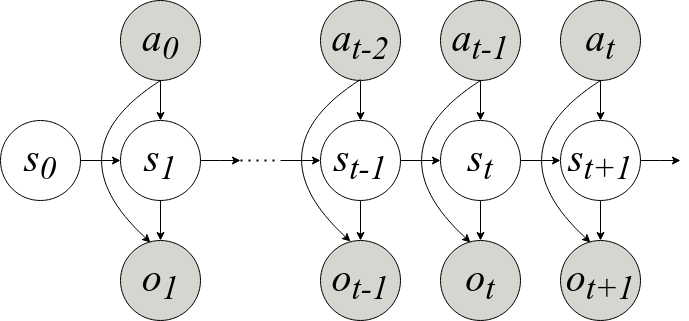
\includegraphics[width=0.4\textwidth]{Images/HMM.png}
	
\end{multicols}


Тогда условие достаточности последнего наблюдения для принятия решения $a_t$  можно описать своими словами следующим образом:     знание о предыдущей истории $h_{t-1}$  не добавит новой информации о распределении $ p(s_t)$ помимо того, что уже известно на основе наблюдения  $o_t$ и предыдущего действия $a_{t-1}$.
Более формально можно выразить с использованием теории информации через понятие относительной взаимной информации, которая определяет, насколько  изменится условная энтропия  состояния $s_t$

\begin{align*} \label{mutualinfo}
\operatorname{I}(s_t;h_{t-1} \mid a_{t-1}, o_t) &\coloneqq \entropy(s_t \mid a_{t-1}, o_t) - \entropy(s_t \mid h_{t-1}, a_{t-1}, o_t)  \\
 &=\KL(p(s_t, h_{t-1} \mid  a_{t-1}, o_t) \parallel p(s_t \mid  a_{t-1}, o_t)p( h_{t-1} \mid  a_{t-1}, o_t))
\end{align*}

В соответствии со свойствами расстояния Кульбака — Лейблера, выражение \ref{mutualinfo}  и указанная в нем относительная взаимная информация равно нулю  тогда для всех $s_t, h_{t-1}, a_{t-1}, o_t$ верно $p(s_t, h_{t-1} \mid  a_{t-1}, o_t) = p(s_t \mid  a_{t-1}, o_t)p( h_{t-1} \mid  a_{t-1}, o_t)$, что равнозначно
\begin{equation}
\label{cond_independ_obs_hist}  p(s_t \mid h_{t-1}, a_{t-1}, o_t ) = p(s_t \mid a_{t-1}, o_t  ), 
\end{equation}
или выражая через множества случайных величин, $ p(A \mid B,C) = p(A \mid C)  $, что обозначается понятием условной независимости наборов случайных величин $A$ и $B$ по набору $C$.
Это в свою очередь выполняется, если в соответствующем графе множество вершин $C$ разделяет $A$ и $B$, для чего множество вершин $C$ должно блокировать все пути из любой вершины, принадлежащей $A$ в любую вершину, принадлежащую $B$ (путь рассматривается для соответствующего неориентированного графа). Блокированием пути $p$ множеством вершин $C$ называется выполнение одного из следующих условий:
\begin{itemize}
	\item  $p$  содержит цепь ${\displaystyle a\to c\to b}$  или разветвление  ${\displaystyle a\gets c\to b}$ такие, что $c$ принадлежит  $C$; или
	\item $p$  содержит инвертированное разветвление   ${\displaystyle a\to \overline c\gets b}$, такое, что ни $\overline c$, ни ее потомок не принадлежит  $C$.
\end{itemize}
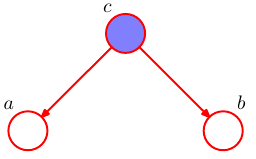
\includegraphics[width=0.25\textwidth]{Images/dsepar1.png}
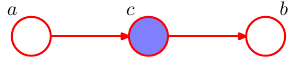
\includegraphics[width=0.25\textwidth]{Images/dsepar2.png}
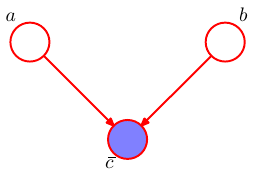
\includegraphics[width=0.25\textwidth]{Images/dsepar3.png}

Графовая модель PoMDP позволяет сделать вывод о невыполнении условий d-разделенности  $A$ и $B$ множеством вершин $C$ (ни один из путей из $A$ в $B$ --- например, $s_t \gets s_{t-1 } \to o_{t-1}$ --- не блокируется множеством $C$), а, следовательно, и том, что равенство \eqref{cond_independ_obs_hist} в общем случае неверно.

Встает вопрос ---  возможно ли вместо оценки доверия по всей истории рекурсивно ее обновлять подобно обновлению истории \eqref{update_history}? В Байесовской статистике для обновления вероятностей оцениваемого параметра $\theta$, являющихся, как было отмечено выше, степенью доверия, после получения новых данных $\mathcal{D}$ используется теорема Байеса
$$p(\textcolor{red}\theta \mid \textcolor{blue}{\mathcal{D}})
 = \frac{p({\mathcal{D}}\mid\theta)p(\theta)}{p(\mathcal{D})}
  \propto p(\textcolor{blue}{\mathcal{D}} \mid \textcolor{red}\theta)p(\textcolor{red}\theta)$$.
На основе указанной теоремы строится процедура рекурсивной Байесовской оценки (Recursive Bayesian estimation, Recursive Bayesian filter), позволяющая обновлять значение belief state с точностью до нормализующей константы:


\begin{align*}
 b_{t+1} &= p(s_{t+1}\mid h_{t+1} )  \\
  &= p(\textcolor{red}{s_{t+1}}\mid \textcolor{blue}{o_{t+1}}, a_t, h_t,)\\
  &= \{ \text{здесь оцениваемым параметром } \theta \text{ является } s_{t+1}, \text{ а новыми данными  } \mathcal{D} \text{ является } o_{t+1} \} = \\
  &\propto p(\textcolor{blue}{o_{t+1}} \mid \textcolor{red}{s_{t+1}}, a_t, h_t) p(\textcolor{red}{s_{t+1}} \mid a_t, h_t) =\\
  &= \{\text{по марковости MDP и формуле полной вероятности}\} =\\
   &= p(\textcolor{blue}{o_{t+1}} \mid \textcolor{red}{s_{t+1}}, a_t) \Bigr[\sum_{s_t}p(\textcolor{red}{s_{t+1}} \mid  s_t, a_t ,h_t)p(s_t|a_t,h_t)\Bigr] =\\
  &= \{\text{состояние не зависит от действия, стоящего в траектории  после состояния } p(s_t|a_t,h_t)=p(s_t|h_t)=b_t\} =\\
  &= p(\textcolor{blue}{o_{t+1}} \mid \textcolor{red}{s_{t+1}}, a_t) \Bigr[\sum_{s_t}p(\textcolor{red}{s_{t+1}} \mid s_t, a_t)b_t \Bigr] 
\end{align*}

То, что belief state является аналогом состояния $s$ наблюдаемого MDP, можно понять, попробовав обобщить понятие состояние.  Для рассмотрения генезиса понятия состояния следует рассмотреть анализируемый процесс как процесс, порождаемый стохастической системой "вход/выход". Модель такой системы представляет из себя черный ящик (black box), который в каждый момент времени $t$ в ответ на контролируемое воздействие (вход) $A_t$ генерирует наблюдение $Y_t$ (выход) и награду $R_t$ и вообще не обладает состоянием. Стохастичность зависимости между входом и выходом обеспечивается случайным входным возмущением $W_t$. 

$$Y_t = f_t(A_{1:t}, W_{1:t})$$
$$R_t = r_t(A_{1:t}, W_{1:t})$$

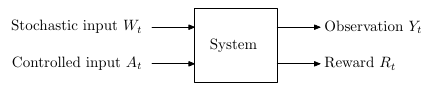
\includegraphics[width=0.6\textwidth]{Images/stochastic_io_system.png}можно


Для PoMDP стратегия имеет вид $\pi(a_t \mid h_t), a \HM\in \A, o \HM\in \mathcal{O}$.

\section{Стохастическая игра}



\end{document}